\documentclass[11pt]{article}
\usepackage{graphicx}
\usepackage{amsthm}
\usepackage{amsmath}
\usepackage{amssymb}
\usepackage[shortlabels]{enumitem}
\usepackage[margin=1in]{geometry}
\graphicspath{{img}}

\newenvironment{solution}
  {\renewcommand\qedsymbol{$\blacksquare$}\begin{proof}[Solution]}
  {\end{proof}}

\setlength\parindent{0pt}

\begin{document}

	\hrule
	\begin{center}
        \textbf{STAT111: Mathematical Statistics II}\hfill \textbf{Spring 2024}\newline

		{\Large Homework 4}

		David Yang
	\end{center}

\hrule

\vspace{1em}

\begin{enumerate}
    \item \textbf{Suppose $V_1$ and $V_2$ are independent $\mathrm{Gamma}(1, \lambda)$ random variables that represent waiting
    times in a Poisson process with rate $\lambda$ events per unit time. Let $X = V_1$ be the time of the
    first event and let $Y = V_1 + V_2$ be the time of the second event.}

    \begin{enumerate}[a)]
      \item \textbf{Find the joint CDF for $X$ and $Y$: $F_{xy}(x, y) = P(X \leq x, Y \leq y)$. Hint: Graph the positive quadrant of the plane
      with axes $V_1$ and $V_2$, and mark the region where $V_1 \leq x$ and $V_1 + V_2 \leq y$. Integrate the joint pdf for $V_1$ and $V_2$ over this region to obtain the function $F_{xy}(x, y)$.
      Note that if there are restrictions on the arguments $x$ and $y$ that you do not specify, then you have failed to define the function.} 

      \begin{solution}
      Note that since $X = V_1$ and $Y = V_1 + V_2$, then 
      \[
        F_{xy}(x, y) = P(X \leq x, Y \leq y) = P(V_1 \leq x, V_1 + V_2 \leq y) = P(V_1 \leq x, V_2 \leq y - V_1)
      \]
      with the restriction that $x \leq y$. \\

      Graphing the positive quadrant of the plane with axes $V_1$ and $V_2$ and integrating the joint pdf for $V_1$ and $V_2$ over the region where $V_1 \leq x$ and $V_1 + V_2 \leq y$ for $x < y$ (shaded),
      \vspace{-0.5cm}
      \begin{center}  
      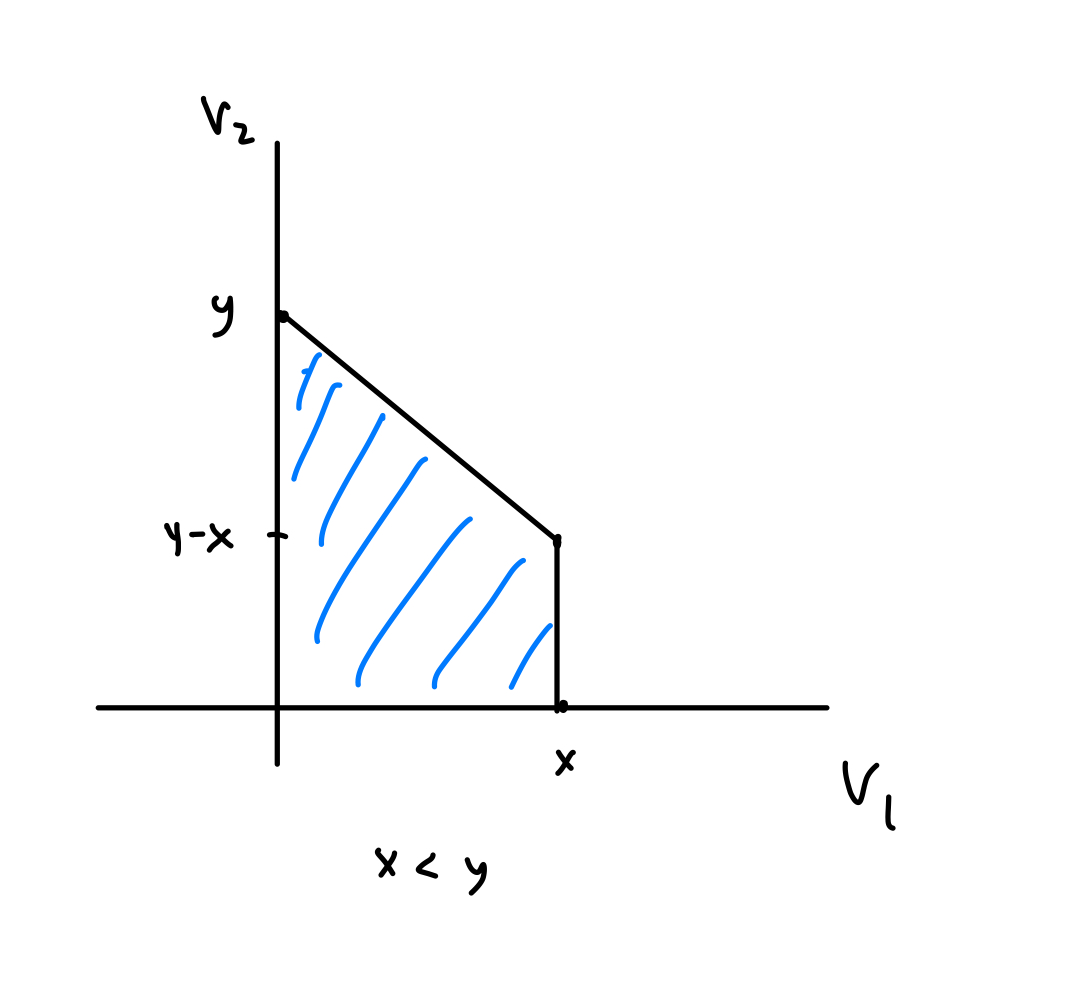
\includegraphics[scale = 0.125]{hw4_p1.jpeg}
      \end{center}
      \vspace{-1cm}
      we see that
      
      \begin{align*}
        F_{xy}(x, y) &= \int_0^x \int_0^{y - V_1} \left( \lambda e^{-\lambda V_1} \right) \left( \lambda e^{-\lambda V_2} \right) dV_2 \, dV_1 \\
        &= \int_0^x \left[ -\lambda e^{-\lambda(V_1 + V_2)} \right]_0^{y-V_1} \, dV_1 \\
        &= \int_0^x -\lambda e^{-\lambda y} + \lambda e^{-\lambda V_1} \, dV_1 \\
        &= \left[ -V_1 \lambda e^{-\lambda y} - e^{-\lambda V_1} \right]_0^x \\
        &= 1 - e^{-\lambda x} - \lambda xe^{-\lambda y},
      \end{align*}
      so the joint CDF for $X$ and $Y$ (with the extra restriction $0 < x < y$) is
      \[
        \boxed{F_{xy}(x, y) = I(0 < x < y) \left(1 - e^{-\lambda x} - \lambda xe^{-\lambda y}\right)}. \qedhere
      \]
    \end{solution}
      \item \textbf{Show how to get the marginal CDF $F_x$ by taking the upper limit for $y$, and $F_y$ by taking the upper limit for $x$. Differentiate each marginal CDF to get the marginal pdfs.}
      \begin{solution}
      There are no restrictions on $y$, so the marginal CDF $F_x$ is simply
      \begin{align*}
        F_x(x) &= \lim_{y \to \infty} I(0 < x < y) \left(1 - e^{-\lambda x} - \lambda xe^{-\lambda y}\right) \\
        &= \boxed{1 - e^{-\lambda x}}.
      \end{align*}

      Differentiating, we get the marginal pdf
      \[
        \boxed{f_x(x) = \lambda e^{-\lambda x}}
      \]
      which intuitively is the pdf for a $\mathrm{Gamma}(1, \lambda)$ random variable. \\

      On the other hand, the upper limit for $x$ is $y$, as $0 < x < y$. Thus, the marginal CDF $F_y$ is
      \begin{align*} 
        F_y(y) &= \lim_{x \to y} I(0 < x < y) \left(1 - e^{-\lambda x} - \lambda xe^{-\lambda y}\right) \\
        &= \boxed{1 - e^{-\lambda y} - \lambda ye^{-\lambda y}}
      \end{align*}

      Differentiating, we can get the marginal pdf
      \begin{align*}
        f_y(y) &= \frac{d}{dy} \left( 1 - e^{-\lambda y} - \lambda ye^{-\lambda y} \right) \\
        &= \lambda e^{-\lambda y} - \lambda e^{-\lambda y} + \lambda^2 y e^{-\lambda y} \\
        &= \boxed{\lambda^2 y e^{-\lambda y}}
      \end{align*}

      which intuitively is the pdf for a $\mathrm{Gamma}(2, \lambda)$ random variable. 
      \end{solution}

      \item \textbf{Show that taking partial derivatives of $F_{xy}$ with respect to $x$ and $y$ yields the joint pdf:}
      \[
        \frac{\partial^2}{\partial x \partial y}F_{xy}(x, y) = \lambda^2 e^{-\lambda y}I(0< x < y). 
      \]

      \begin{solution}
      Finally, we can derive the joint pdf. Note that
      \begin{align*}
        f_{xy}(x, y) = \frac{\partial^2}{\partial x \partial y}F_{xy}(x, y) &= \frac{\partial}{\partial x}\left( \frac{\partial}{\partial y} F_{xy}(x, y)\right) \\
        &= \frac{\partial}{\partial x}\left( \frac{\partial}{\partial y} F_{xy}(x, y)\right) \\
        &= \frac{\partial}{\partial x}\left( \frac{\partial}{\partial y}  \left( I(0 < x < y) \left(1 - e^{-\lambda x} - \lambda xe^{-\lambda y}\right) \right)\right) \\
        &= \frac{\partial}{\partial x}\left( I(0 < x < y) \lambda^2 xe^{-\lambda y} \right) \\
        &= \boxed{\lambda^2 e^{-\lambda y}I(0 < x < y)}
      \end{align*}

      as desired.
      \end{solution}
    \end{enumerate}

    \newpage

    \item \textbf{Suppose $Z_1$ and $Z_2$ have joint pdf}
    \[
      f_{12}(z_1, z_2) = \exp \left[ -\log (\pi ) - 2(z_1^2 + z_2^2 + \sqrt{3}z_1 z_2) \right].
    \]
    \begin{enumerate}[a)]
      \item \textbf{Identify this as a bivariate Normal density by specifying the means $\mu_1$ and $\mu_2$, standard deviations $\sigma_1$ and $\sigma_2$, and the correlation $ \rho $.}
      
      \begin{solution}
        Note that 
        \begin{align*}
          f_{12}(z_1, z_2) &= \exp \left[ -\log (\pi ) - 2(z_1^2 + z_2^2 + \sqrt{3}z_1 z_2) \right] \\
          &= \frac{1}{\pi} \exp \left[ - 2(z_1^2 + z_2^2 + \sqrt{3}z_1 z_2) \right].
        \end{align*}

        Rewriting this expression, we have that 
        \begin{align*}
          f_{12}(z_1, z_2) &= \frac{1}{\pi} \exp \left[ - 2(z_1^2 + z_2^2 + \sqrt{3}z_1 z_2) \right] \\
          &= \frac{1}{2\pi \left( \frac{1}{2} \right)}  \exp \left[ -\frac{1}{2\left( \frac{1}{4} \right) }\left(z_1^2 + z_2^2 - 2\left( -\frac{\sqrt{3}}{2} \right) z_1 z_2 \right) \right].
        \end{align*}

        We recognize this as a bivariate Normal density, with 
        \[
          \boxed{\mu_1 = \mu_2 = 0, \sigma_1 = \sigma_2 = 1, \text{ and } \rho = -\frac{\sqrt{3}}{2}}. \qedhere
        \]
      \end{solution}

      \item \textbf{Any joint pdf may be expressed as a marginal pdf multiplied by a conditional pdf. Show that $f_{12}(z_1, z_2)$ may be written as the product of a standard Normal density for $Z_1$ and a Normal density for $Z_2\mid z_1$ that depends on $z_1$.
      Give the conditional mean and variance for $Z_2 \mid z_1$ and show that they agree with the formulas $\mathbb{E}[Z_2 \mid z_1] = \beta_0 + \beta_1 z_1$ with $\beta_1 = \rho \frac{\sigma_2}{\sigma_1}$, 
      $\beta_0 = \mu_2 - \beta_1 \mu_1$, and $\mathrm{Var} \left[Z_2 \mid z_1 \right] = (1-\rho^2)\sigma_2^2$.}

      \begin{solution}
      Let $Z_1 \sim N(0, 1)$. We know that $f_{Z_1}(z_1) = \frac{1}{\sqrt{2\pi}} \exp \left[ -\frac{z_1^2}{2} \right].$ 
      \begin{align*}
        f_{12}(z_1, z_2) &= \frac{1}{\pi} \exp \left[- 2(z_1^2 + z_2^2 + \sqrt{3}z_1 z_2) \right] \\
        &= \frac{1}{\sqrt{2\pi}} \exp \left[ -\frac{z_1^2}{2} \right] \frac{\sqrt{2}}{\sqrt{\pi}} \exp \left[- \left(\frac{3}{2}z_1^2 + 2z_2^2 + 2\sqrt{3}z_1 z_2\right) \right] 
      \end{align*}
      Recognizing the first term as $f_{Z_1}(z_1)$, the pdf for $Z_1$, we have that
      \[
        f_{12}(z_1, z_2) = f_{Z_1}(z_1) \frac{\sqrt{2}}{\sqrt{\pi}} \exp \left[- \left(\frac{3}{2}z_1^2 + 2z_2^2 + 2\sqrt{3}z_1 z_2\right) \right].
      \]

      Rearranging the second term and simplifying, we get that
      \begin{align*}
        f_{12}(z_1, z_2) &= f_{Z_1}(z_1) \frac{\sqrt{2}}{\sqrt{\pi}} \exp \left[- \left(\frac{3}{2}z_1^2 + 2z_2^2 + 2\sqrt{3}z_1 z_2\right) \right] \\
        &= f_{Z_1}(z_1) \frac{\sqrt{2}}{\pi} \exp \left[ -2\left(z_2^2 + \sqrt{3}z_1z_2 + \frac{3}{4}z_1^2  \right)\right] \\
        &= f_{Z_1}(z_1) \frac{1}{\sqrt{2\pi \cdot \frac{1}{4}}} \exp \left[ -\frac{\left( z_2 + \frac{\sqrt{3}}{2}z_1 \right)^2 }{2\left( \frac{1}{4} \right) }\right].
      \end{align*}

      We recognize the second term now as the pdf for $Z_2 \mid z_1 \sim N\left( -\frac{\sqrt{3}}{2}z_1, \frac{1}{4} \right)$, so we conclude
      \[
        f_{12}(z_1, z_2) = f_{Z_1}(z_1) f_{Z_2 \mid z_1}(z_2 \mid z_1).
      \] 
      Note that $\mathbb{E}\left[Z_2 \mid z_1 \right] = -\frac{\sqrt{3} }{2}z_1$, and 
      \begin{align*}
        \beta_0 + \beta_1 z_1 &= \left(\mu_2 - \left(\rho \frac{\sigma_2}{\sigma_1}\right)\mu_1\right) + \rho \frac{\sigma_2}{\sigma_1}z_1 \\
        &= (0 - 0) - \frac{\sqrt{3}}{2}z_1 \\
        &= -\frac{\sqrt{3} }{2} z_1.
      \end{align*}

      Similarly, $\mathrm{Var} \left[Z_2 \mid z_1 \right] = \frac{1}{4}$ and 
      \begin{align*}
        \left( 1 - \rho^2 \right) \sigma_2^2 &= \left( 1 - \left( -\frac{\sqrt{3}}{2} \right)^2\right) 1^2 \\
        &= \frac{1}{4},
      \end{align*}
      matching the results from the given formulas.
      \end{solution}

      \item \textbf{You can also show conditional results using representation. For $Z_o \sim N(0, 1)$ independent of $Z_2$, define $Z_1 = \rho Z_2 + \sqrt{1-\rho^2}Z_o$ to have correlation $\rho$ with $Z_2$.
      Show that conditioning on $Z_2 = z_2$ and treating this as constant in the representation of $Z_1$ results in a conditional distribution $Z_1 \mid z_2$ that mirrors that of $Z_2 \mid z_1$ from part (b).}
    
      \begin{solution}
        For $Z_o \sim N(0, 1)$ independent of $Z_2$, define $Z_1 = \rho Z_2 + \sqrt{1-\rho^2}Z_o$ as stated. Note that $\sqrt{1-\rho^2}Z_o \sim N(0, 1-\rho^2)$. Conditioning on $Z_2 \mid z_2$, we find that
        \[
          Z_1 \mid z_2 \sim N(\rho Z_2, 1-\rho^2)
        \] 
        For $\rho = -\frac{\sqrt{3} }{2}$ (giving $1-\rho^2 = \frac{1}{4}$), we have
        \[
          Z_1 \mid z_2 \sim N\left( -\frac{\sqrt{3} }{2}z_2, \frac{1}{4} \right) 
        \]
        which matches the distribution of $Z_2 \mid z_1$ in part (b).
      \end{solution}
    \end{enumerate}

    \newpage
    
    \item \textbf{Suppose $X$ and $Y$ have joint pdf $f_{xy}(x, y) = I(0 < x < 1, -x < y < x)$.}
    \begin{enumerate}[a)]
      \item \textbf{Explain how you can tell, without finding the marginal densities, that the conditional densities are Uniform.
      Write out the conditional densities $f_{x \mid y}(x \mid y)$ and $f_{y \mid x}(y \mid x)$.}

      \begin{solution}
      The conditional densities are uniform as they are proportional to the joint density, which can be thought of as Uniform (as it is an indicator variable). \\

      Since by construction, $|y| < x$ and $x < 1$ it follows that the conditional density is
      \[
        f_{x \mid y}(x \mid y) = \frac{1}{1 - |y|} I(|y| < x < 1).
      \]
      Similarly, we must have that $-x < y < x$, so
      \[
        f_{x \mid y}(y \mid x) = \frac{1}{2x} I(-x < y < x). \qedhere
      \]\end{solution}
      \item \textbf{Explain how you can tell, without finding the marginal densities, that $X$ and $Y$ are not independent. Find the marginal pdf's $f_x(x)$ and $f_y(y)$ 
      and verify that $f_{xy}(x, y) \neq f_x(x)f_y(y)$.}

      \begin{solution}
      Note that very clearly, $f_{x \mid y}(x, y)$ are not equal for different values of $y$, so $X$ and $Y$ cannot be independent. We can verify this with the marginal pdfs:
      \[
        f_x(x) = \frac{f_{xy}(x, y)}{f_{y \mid x}(y \mid x)} = \frac{I(0 < x < 1, -x < y, x)}{\frac{1}{2x} I(-x < y < x)}= 2x I(0 < x < 1).
      \]
      Similarly, 
      \[
        f_x(y) = \frac{f_{xy}(x, y)}{f_{x \mid y}(x \mid y)} = \frac{I(0 < x < 1, -x < y, x)}{\frac{1}{1 - |y|} I(|y| < x < 1)}= (1- |y|) I(-1 < y < 1).
      \]

      We check that
      \begin{align*}
        f_X(x)f_Y(y) &= 2x(1-|y|) I(0 < x < 1) I(-1 < y < 1) \\
        &\neq I(0 < x < 1, -x < y, x) = f_{XY}(x, y)
      \end{align*}
      confirming that $X$ and $Y$ are not independent.
      \end{solution}

      \item \textbf{Show that $X$ and $Y$ are uncorrelated.}
      
      \begin{solution}
      Note that
      \[
        \mathbb{E}\left[XY \right] = \int_0^1 \int_{-x}^x xy I(0 < x < 1, -x < y < x) \, dy \, dx = 0
      \]
      by symmetry. Similarly,
      \[
        \mathbb{E}\left[X \right] = \int_0^1 x(2x) \, dx = 1
      \]
      and 
      \[
        \mathbb{E}\left[Y \right] = \int_{-1}^1 y(1 - |y|) \, dy = 0
      \]
      by symmetry. Thus, we have that
      \[
        \mathbb{E}\left[XY \right] - \mathbb{E}\left[X \right] \mathbb{E}\left[Y \right] = 0
      \]
      so $X$ and $Y$ are uncorrelated, as desired.
      \end{solution}
    
    \end{enumerate}

    \newpage
    \item 
    \begin{enumerate}[a)]
      \item \textbf{Suppose $X_1$ and $X_2$ are Bernoulli random variables with expectations $p_1$ and $p_2$. Show that $X_1$ and $X_2$ are independent if and only if they are uncorrelated.
      This shows the Bernoulli distribution is special like the multivariate Normal distribution in that uncorrelated implies independence.}
      
      \begin{solution}
      Note that if $X_1$ and $X_2$ are independent, then we have that $P(X_1 = 1, X_2 = 1) = P(X_1 = 1)P(X_2 = 1)$. Note that
      \[
        X_1 X_2 = \begin{cases}
          1 &\text{ if $X_1 = 1$ and $X_2 = 1$}  \\
          0 &\text{ otherwise}
        \end{cases}
      \]
      so $\mathbb{E}\left[X_1 X_2 \right] = P(X_1 = 1, X_2 = 1) = P(X_1 = 1)P(X_2 = 1) = \mathbb{E}\left[X_1 \right]\mathbb{E}\left[X_2 \right]$. \\
      
      Thus,
      \[
        \mathbb{E}\left[X_1 X_2 \right] = \mathbb{E}\left[X_1 \right] \mathbb{E}\left[X_2 \right] 
      \]
      and so $X_1$ and $X_2$ are uncorrelated. \\

      On the other hand, suppose that $X_1$ and $X_2$ are independent, so that $\mathbb{E}\left[X_1 X_2 \right] = \mathbb{E}\left[X_1 \right] \mathbb{E}\left[X_2 \right] = p_1 p_2$. \\

      By the Law of Total Probability, we have that
      \[
        P(X_1 = 1) = P(X_1 = 1 \mid X_2 = 1)P(X_2 = 1) + P(X_1 = 1 \mid X_2 = 0)P(X_2 = 0).
      \]
      Since $P(X_1 = 1) = \mathbb{E}\left[X_1 \right] = p_1$, $P(X_1 = 1 \mid X_2 = 1)P(X_2 = 1) = \mathbb{E}\left[X_1 X_2 \right] = p_1 p_2$, and $P(X_2 = 0) = 1 - \mathbb{E}\left[X_2 \right] = 1-p_2$, we must have that
      \begin{align*}
        P(X_1 = 1 \mid X_2 = 0) &= \frac{P(X_1 = 1) - P(X_1 = 1 \mid X_2 = 1)}{P(X_2 = 0)} \\
        &= \frac{p_1 - p_1 p_2}{1 - p_2} \\
        &= p_1.
      \end{align*}

      Similarly, by the Law of Total Probability, we have that
      \[
        P(X_2 = 1) = P(X_2 = 1 \mid X_1 = 1)P(X_1 = 1) + P(X_2 = 1 \mid X_1 = 0)P(X_1 = 0)
      \]

      and so 
      \begin{align*}
        P(X_2 = 1 \mid X_1 = 0) &= \frac{P(X_2 = 1) - P(X_2 = 1 \mid X_1 = 1)}{P(X_1 = 0)} \\
        &= \frac{p_2 - p_1 p_2}{1 - p_1} \\
        &= p_2.
      \end{align*}

      We see that both $P(X_1 = 1) = P(X_1 = 1 \mid X_2 = 1) = P(X_1 = 1 \mid X_2 = 0) = p_1$ and 
      $P(X_2 = 1) = P(X_2 = 1 \mid X_1 = 1) = P(X_2 = 1 \mid X_1 = 0) = p_2$. \\
      
      Through a similar line of reasoning, we can
      conclude that $P(X_1 = 0) = P(X_1 = 0 \mid X_2 = 1) = P(X_1 = 0 \mid X_2 = 1) = 1 - p_1$ and 
      $P(X_2 = 0) = P(X_2 = 0 \mid X_1 = 1) = P(X_2 = 0 \mid X_1 = 0) = 1 - p_2$. \\

      Thus, $X_1$ and $X_2$ are independent, as desired. \\
    
      It follows that $X_1$ and $X_2$ are independent if and only if they are uncorrelated, as desired. \end{solution}
      
      \item \textbf{Suppose $Y = X_1 + X_2$ with $X_1$ and $X_2$ independent. If you learn that $Y$ and $X_1$ are
      Normal variables, prove that $X_2$ is also a Normal random variable.} 

      \begin{solution}
      Suppose that $Y \sim N(\mu_Y, \sigma_Y^2)$ and $X_1 \sim N(\mu_1, \sigma_1^2)$. Since $Y = X_1 + X_2$, we know that the MGF of $Y$ and $X_1 + X_2$ are the same, so
      \[
        M_{X_1 + X_2}(t) = M_Y(t)
      \]
      meaning that $M_{X_1}(t) M_{X_2}(t) = M_Y(t)$ and 
      \[
        M_{X_2}(t) = \frac{M_Y(t)}{M_{X_1}(t)}.
      \]
      Since $Y \sim N(\mu_Y, \sigma_Y^2)$ and $X_1 \sim N(\mu_1, \sigma_1^2)$, we know that 
      \[
        M_Y(t) = e^{t \mu_Y + \frac{1}{2}\sigma_Y^2 t^2} \text{ and } M_{X_1}(t) = e^{t \mu_1 + \frac{1}{2}\sigma_1^2 t^2}.
      \]
      Thus,
      \begin{align*}
        M_{X_2}(t) &= \frac{M_Y(t)}{M_{X_1}(t)} \\
        &= \frac{e^{t \mu_Y + \frac{1}{2}\sigma_Y^2 t^2}}{e^{t \mu_1 + \frac{1}{2}\sigma_1^2 t^2}} \\
        &= e^{t(\mu_Y - \mu_1) + \frac{1}{2}(\sigma_Y^2 - \sigma_1^2)t^2}
      \end{align*}
      which is the MGF of the Normal random variable $N(\mu_Y - \mu_1, \sigma_Y^2 - \sigma_1^2)$. \\

      Thus, if $Y$ and $X_1$ are Normal variables and $Y = X_1 + X_2$ with $X_1$ and $X_2$ independent, it follows that $X_2$ is also a Normal random variable.
      \end{solution}
    \end{enumerate}
    
\end{enumerate}

\end{document}
